\documentclass[11pt,a4paper]{article}
\usepackage[a4paper,margin=2.5cm]{geometry}
\usepackage{amsmath,amssymb,amsthm}
\usepackage{graphicx}
\usepackage{booktabs}
\usepackage{longtable}
\usepackage{array}
\usepackage{hyperref}
\usepackage{xcolor}
\usepackage{listings}
\usepackage{enumitem}
\usepackage{parskip}
\usepackage{fancyhdr}
\usepackage{titlesec}

\hypersetup{
  colorlinks=true,
  linkcolor=blue!50!black,
  citecolor=blue!50!black,
  urlcolor=blue!50!black,
  pdftitle={ozGUI / ozLib: Ornstein--Zernike Solver Toolkit},
  pdfauthor={ozGUI/ozLib project}
}

\lstset{
  basicstyle=\ttfamily\small,
  breaklines=true,
  frame=single,
  columns=fullflexible,
  backgroundcolor=\color{gray!8},
  keywordstyle=\color{blue!60!black},
  commentstyle=\color{green!40!black},
  stringstyle=\color{red!60!black},
  language=Python,
  showstringspaces=false
}

\pagestyle{fancy}
\fancyhf{}
\fancyhead[L]{ozGUI / ozLib Documentation}
\fancyhead[R]{\thepage}
\renewcommand{\headrulewidth}{0.4pt}

\newtheorem{remark}{Remark}

\newcommand{\code}[1]{\texttt{#1}}

\title{\textbf{ozGUI / ozLib}\\[0.3cm]
\large A Python Toolkit for Solving the Ornstein--Zernike Equation\\[0.2cm]
\normalsize Theory, Formulas, and Usage Reference}
\author{}
\date{\today}

\begin{document}
\maketitle
\thispagestyle{empty}

\begin{abstract}
\noindent
This document is the reference manual for \code{ozGUI} and \code{ozLib}, a Python
re-implementation of SASfit's Ornstein--Zernike (OZ) equation solver
(\code{src/sasfit\_oz/} in the SASfit source tree). It documents, with exact
mathematical formulas, every interaction potential, every closure relation, and
every numerical solver algorithm currently implemented, together with the
underlying Hankel-transform-based discretisation scheme and the two ways of
using the toolkit: as an interactive Tkinter GUI (\code{ozGUI.py}) and as a plain
importable Python library (\code{ozLib.py}). Formulas throughout were ported and
verified directly against SASfit's own C source
(\code{src/sasfit\_oz/sasfit\_oz\_solver.c}, \code{src/plugins/*}), and, where an
independent literature source was available, cross-checked against it as well;
deviations, known limitations, and one deliberately-excluded closure are
documented explicitly rather than silently omitted.
\end{abstract}

\tableofcontents
\clearpage

\section{Overview}

\code{ozGUI}/\code{ozLib} solves the Ornstein--Zernike (OZ) integral equation for a
single-component, isotropic fluid of spherically symmetric particles, given
\begin{itemize}[nosep]
  \item a pair interaction potential $U(r)$ (Section~\ref{sec:potentials}),
  \item a closure relation connecting the direct correlation function $c(r)$ to
        the total correlation function $h(r)=g(r)-1$ (Section~\ref{sec:closures}),
  \item a volume fraction $\varphi$, and
  \item a numerical solver algorithm that finds the self-consistent fixed point
        of the resulting nonlinear system (Section~\ref{sec:solvers}).
\end{itemize}
The output is the pair correlation function $g(r)$, the direct correlation
function $c(r)$, the static structure factor $S(q)$, and several auxiliary
quantities (the cavity function $y(r)$, the bridge function $B(r)$, the
indirect correlation function $\Gamma(r)=h(r)-c(r)$, and the reduced potential
$U(r)/k_BT$).

Two front ends share the exact same computational core (\code{ozLib.py}), so
results obtained through either are identical by construction:
\begin{itemize}[nosep]
  \item \textbf{\code{ozGUI.py}} --- an interactive Tkinter application with
        potential/closure/solver dropdowns, a 9-tab plot panel, run history,
        and Save/Load/ASCII/CSV/Excel/PNG export (Section~\ref{sec:gui}).
  \item \textbf{\code{ozLib.py}} --- a plain Python function,
        \code{ozLib.solve(...)}, usable directly in scripts without any GUI
        dependency (Section~\ref{sec:ozlib}).
\end{itemize}

\section{The Ornstein--Zernike Equation and its Discretisation}
\label{sec:theory}

\subsection{The OZ equation}

For an isotropic, single-component fluid the Ornstein--Zernike equation reads,
in real space,
\begin{equation}
  h(r) = c(r) + \rho \int c(|\mathbf{r}-\mathbf{r}'|)\, h(r')\, d\mathbf{r}',
\end{equation}
where $\rho$ is the number density and the convolution is over all space.
Introducing the indirect correlation function $\Gamma(r) \equiv h(r)-c(r)$, and
Fourier--Bessel (Hankel) transforming (exploiting isotropy to reduce the 3D
Fourier transform to a 1D sine transform), the OZ equation becomes purely
algebraic in reciprocal space,
\begin{equation}
  \hat\Gamma(q) = \frac{\hat c(q)}{1-\rho\,\hat c(q)} - \hat c(q),
  \label{eq:oz-fourier}
\end{equation}
where $\hat f(q)$ denotes the (3D, spherically-symmetric) Fourier transform of
$f(r)$. The OZ equation alone relates two unknowns, $c(r)$ and $h(r)$ (or
equivalently $\Gamma(r)$); a second, independent relation --- the
\emph{closure} --- is required to close the system. Every closure implemented
here has the general form
\begin{equation}
  c(r) = f\big(\Gamma(r), U(r)\big)
\end{equation}
for some function $f$ specific to the closure (Section~\ref{sec:closures}). The
full problem is therefore a fixed-point problem in $\Gamma(r)$ (or, in an
equivalent formulation used by some solvers here, in $c(r)$ and $h(r)$
jointly): starting from a trial $\Gamma(r)$, the closure gives $c(r)$, the OZ
equation (Eq.~\ref{eq:oz-fourier}) gives a new $\Gamma(r)$, and a solver
algorithm (Section~\ref{sec:solvers}) drives this map to self-consistency.

\subsection{Discrete grid: real space}

The real-space grid is a plain equal-spaced grid of $N=\code{numberOfRadialSamplingPoints}$
points,
\begin{equation}
  r_i = i\,\Delta r, \qquad i=1,2,\dots,N,
\end{equation}
starting at $\Delta r$ rather than $0$ (division by $r$ appears in the Hankel
transform below, so $r=0$ is avoided by construction rather than special-cased).
The hard-core diameter $\sigma$ is placed at grid index
$\code{hardSphereRadiusInPoints}$ (called $n_\sigma$ below), i.e.
\begin{equation}
  \sigma = n_\sigma\,\Delta r, \qquad
  \text{total range } r_{\max} = (N-1)\Delta r = \frac{N-1}{n_\sigma}\,\sigma.
\end{equation}
Both $N$ and $n_\sigma$ are configurable (constructor keyword arguments
\code{numberOfRadialSamplingPoints}, \code{hardSphereRadiusInPoints} on every
solver class, and identically-named arguments on \code{ozLib.solve()}); the
historical defaults are $N=4096$, $n_\sigma=100$, giving $r_{\max}\approx
41\,\sigma$ and $\Delta r = 0.01\,\sigma$. Increasing $N$ at fixed $n_\sigma$
extends the range without losing near-contact resolution --- important for
slowly-decaying, long-range potentials (e.g.\ small-$\kappa$ Yukawa/DLVO tails),
where a too-short grid truncates the potential before it has actually decayed
to zero, distorting $S(q)$ at low $q$ (this was verified directly: a 4$\times$
extension of the default grid reduced a Yukawa potential's residual value at
the grid edge from $\mathcal{O}(10^{-4})\,k_BT$ to $\mathcal{O}(10^{-10})\,k_BT$,
and changed $S(q\!\to\!0)$ by about 33\%).

\subsection{Discrete Hankel transform}

For an isotropic function $f(r)$ the 3D Fourier transform reduces to
\begin{equation}
  \hat f(q) = \frac{4\pi}{q}\int_0^\infty r\,f(r)\,\sin(qr)\,dr,
\end{equation}
which is implemented here as a type-I discrete sine transform (DST) of
$r_i f(r_i)$, following the same construction documented in SASfit's own
theory notes (equations 5.18/5.19 there):
\begin{equation}
  \hat f(q_k) = \frac{2\pi \Delta r^2}{\Delta q}\cdot
                \frac{\mathrm{DST\text{-}I}\big[r_i f(r_i)\big]_k}{k},
  \qquad
  \Delta q = \frac{\pi}{(N+1)\Delta r},
  \qquad q_k = k\,\Delta q.
\end{equation}
The inverse transform is the same operation up to a normalisation factor
($\Delta q^3/[(2\pi)^3\Delta r^3]$), since the Hankel transform pair is (up to
constants) self-inverse. Both directions are implemented once, in
\code{OZfixpointOperator.hankelTransform()}/\code{inverseHankelTransform()},
and shared by every closure and every solver.

\subsection{Grand-canonical thermodynamic quantities}

For the hard-sphere/Percus--Yevick case, the exact grand-canonical
compressibility-route structure factor at $q=0$ is available in closed form
(used as an internal consistency check, e.g.\ in RMSA's own bisection, see
Section~\ref{sec:rmsa-closure}):
\begin{equation}
  S(q\!=\!0) = \frac{(1-\varphi)^4}{(1+2\varphi)^2}.
\end{equation}

\section{Interaction Potentials}
\label{sec:potentials}

Every potential is specified through its Boltzmann factor
$\exp[-U(r)/k_BT]$ (stored as \code{boltzmannOfP2Ppotential}), evaluated on the
grid described above; all energies are in $k_BT$ units and all lengths in units
where the hard-core diameter is $\sigma=n_\sigma\Delta r$. Potentials that
support the repulsive/attractive potential split needed by
switching-function closures (Rogers--Young, HMSA, and the Gstar-based bridge
closures of Section~\ref{sec:closures}) additionally populate
\code{repulsivePartOfP2Ppotential}/\code{attractivePartOfP2Ppotential}. All 17
potentials below are available via \code{setPotentialByName(name, *args)} or
directly as \code{set<Name>Potential(...)}.

\subsection{Hard Sphere}
\begin{equation}
  \exp[-U(r)/k_BT] = \begin{cases} 0 & r<\sigma \\ 1 & r\ge\sigma. \end{cases}
\end{equation}

\subsection{Lennard-Jones}
\begin{equation}
  U(r)/k_BT = 4\varepsilon\left[\left(\frac{\sigma}{r}\right)^{12}-\left(\frac{\sigma}{r}\right)^{6}\right],
\end{equation}
with $\varepsilon$ in $k_BT$ units. The potential is split at its minimum
($r_{\min}=2^{1/6}\sigma$) into a repulsive part ($r<r_{\min}$) and an
attractive part ($r\ge r_{\min}$), for use by switching-function closures.

\subsection{Yukawa (screened Coulomb), with optional hard core}
\begin{equation}
  U(r)/k_BT = K\,\frac{\sigma}{r}\,e^{-r/\lambda},
\end{equation}
where $\lambda$ is the screening length (in units of $\sigma$) and $K$ the
contact interaction strength; a hard core can optionally be added
(\code{doAddHardSphere}), in which case the exponential and $1/r$ factors are
shifted independently as in SASfit's own construction, and the potential is
set to $\infty$ (Boltzmann factor 0) for $r<\sigma$.

\subsection{Star polymer potential (Likos)}
\begin{equation}
  U(r)/k_BT =
  \begin{cases}
    \dfrac{5}{18}f^{3/2}\left[-\ln\!\dfrac{r}{\sigma}+\dfrac{1}{1+\sqrt{f}/2}\right] & r\le\sigma\\[2ex]
    \dfrac{5}{18}f^{3/2}\,\dfrac{1}{1+\sqrt{f}/2}\,\dfrac{\sigma}{r}\,
      \exp\!\left[-\dfrac{\sqrt{f}(r-\sigma)}{2\sigma}\right] & r>\sigma,
  \end{cases}
\end{equation}
where $f=$ \code{NumberOfArms} is the number of arms of the star polymer.

\subsection{Depletion potential (Oversteegen \& Lekkerkerker)}
Two-sphere overlap-volume depletion potential between big spheres (diameter
$\sigma_1=\sigma$, the species this OZ solve is for) induced by small
depletant spheres (diameter $\sigma_2=$ \code{sigmaRatio}$\cdot\sigma_1$, number
density $\rho_2$ set via the depletant volume fraction \code{phi2}):
\begin{equation}
  U(r)/k_BT = -\rho_2\,\frac{\pi\sigma_1^3(1+r_t)^3}{6}
  \left[1-\frac{3r}{2(1+r_t)\sigma_1}+\frac{r^3}{2(1+r_t)^3\sigma_1^3}\right],
  \qquad \sigma_1\le r<\sigma_1+\sigma_2,
\end{equation}
with $r_t=\sigma_2/\sigma_1$, and $U=0$ for $r\ge\sigma_1+\sigma_2$; hard core
for $r<\sigma_1$.

\subsection{DLVO (electrostatic double-layer + van der Waals)}
\label{sec:dlvo}
\begin{equation}
  U(r)/k_BT = U_{\mathrm{el}}(r) + U_{\mathrm{vdW}}(r), \qquad r>\sigma,
\end{equation}
\begin{equation}
  U_{\mathrm{el}}(r) = \frac{L_B Z^2}{(1+\kappa a)^2}\,\frac{e^{-\kappa(r-\sigma)}}{r},
  \qquad
  U_{\mathrm{vdW}}(r) = -\frac{A}{6}\left[\frac{2a^2}{r^2-4a^2}+2\left(\frac{a}{r}\right)^2
    +\ln\!\left(1-4\Big(\frac{a}{r}\Big)^2\right)\right],
\end{equation}
where $a=\sigma/2$, $\kappa$ the inverse Debye screening length, $Z$ the
macro-ion charge, $L_B$ the Bjerrum length, and $A$ the effective Hamaker
constant. $U_{\mathrm{vdW}}$'s genuine divergence at $r=\sigma$ is excluded from
the computation itself (not merely masked afterward), since the grid places a
real point at exactly $r=\sigma$.

\subsection{DLVO + hydration repulsion}
As Section~\ref{sec:dlvo}, plus a short-range exponential hydration term,
\begin{equation}
  U(r)/k_BT = U_{\mathrm{DLVO}}(r) - 2\,G_{HY}\,e^{-(r-\sigma)/D_H}, \qquad r>\sigma,
\end{equation}
with hydration strength $G_{HY}$ and decay length $D_H$.

\subsection{Fermi distribution model (Likos)}
\begin{equation}
  U(r)/k_BT = \varepsilon\,\frac{1+e^{-\sigma/\xi}}{1+e^{(r-\sigma)/\xi}}.
\end{equation}
The limit $\xi\to0$ reduces to the penetrable sphere model (below), and is
handled as a special case when $\xi=0$ is passed exactly.

\subsection{Generalized Gaussian core model (GGCM-$n$)}
\begin{equation}
  U(r)/k_BT = \varepsilon\,\exp\!\left[-\alpha\left(\frac{r}{\sigma}\right)^{n}\right].
\end{equation}

\subsection{Hard sphere + 3 additive Yukawa tails}
\begin{equation}
  U(r)/k_BT = -\frac{\sigma}{r}\sum_{i=1}^{3} K_i\,\exp\!\left[-\frac{r-\sigma}{\sigma\,\lambda_i}\right], \qquad r\ge\sigma,
\end{equation}
with hard core for $r<\sigma$; each $(K_i,\lambda_i)$ pair may be set to zero to
recover fewer effective Yukawa terms.

\subsection{Ionic microgel (Likos et al.)}
A multi-term analytical potential for a charged microgel sphere of charge $Z$,
dielectric constant $ED$, and inverse screening length $\kappa_\Pi/\sigma$
inside the gel, following Likos et al.\ (2011); the full piecewise expression
(different polynomial/hyperbolic forms inside vs.\ outside the gel radius) is
implemented exactly as in \code{sasfit\_oz\_potential\_ionic\_microgel.c} and is
reproduced verbatim in the source rather than restated here, since it spans
several auxiliary terms without a single compact closed form.

\subsection{Piecewise-constant hard-sphere shoulder/well (3 segments)}
\begin{equation}
  U(r)/k_BT =
  \begin{cases}
    \varepsilon_1 & \sigma\le r<\sigma+\delta_1\\
    \varepsilon_2 & \sigma+\delta_1\le r<\sigma+\delta_1+\delta_2\\
    \varepsilon_3 & \sigma+\delta_1+\delta_2\le r<\sigma+\delta_1+\delta_2+\delta_3\\
    0 & \text{otherwise (outside all three steps)},
  \end{cases}
\end{equation}
hard core for $r<\sigma$; each $\varepsilon_j$ may be positive (shoulder) or
negative (well). This is the general $n=3$ piecewise-constant family used as
an independent cross-check for the RFA analytical solver
(Section~\ref{sec:rfa}).

\subsection{Penetrable sphere model (Likos, Watzlawek, L\"owen)}
\begin{equation}
  U(r)/k_BT = \begin{cases}\varepsilon & r\le\sigma\\ 0 & r>\sigma.\end{cases}
\end{equation}

\subsection{Soft sphere (inverse power law)}
\begin{equation}
  U(r)/k_BT = \varepsilon\left(\frac{\sigma}{r}\right)^{n}.
\end{equation}

\subsection{Parabolic (Hertzian) sphere}
\begin{equation}
  U(r)/k_BT = \begin{cases}\varepsilon\left(1-\dfrac{r}{\sigma}\right)^{5/2} & r\le\sigma\\ 0 & r>\sigma.\end{cases}
\end{equation}

\subsection{Square well}
\label{sec:squarewell-potential}
\begin{equation}
  U(r)/k_BT = \begin{cases} \infty & r<\sigma\\ \varepsilon & \sigma\le r\le\sigma+\delta \\ 0 & r>\sigma+\delta,\end{cases}
\end{equation}
with well width $\delta$ (well outer range $\lambda=1+\delta/\sigma$ in the
notation of Section~\ref{sec:sharma-sharma}); $\varepsilon<0$ for an attractive
well, $\varepsilon>0$ for a repulsive shoulder.

\subsection{Sticky hard sphere (Baxter's adhesive limit)}
\label{sec:stickyhs-potential}
\begin{equation}
  U(r)/k_BT = \begin{cases} \infty & r<\sigma\\ \ln\!\left(\dfrac{12\,\tau\,\delta}{\sigma+\delta}\right) & \sigma\le r\le\sigma+\delta\\ 0 & r>\sigma+\delta,\end{cases}
\end{equation}
using Baxter's stickiness parameter $\tau$ (small $\tau$ = sticky, large $\tau$
= hard-sphere limit) and a finite well width $\delta$ --- the same $\tau$
convention as SASfit's own \code{robertus\_shs} plugin, giving a natural point
of comparison between this (monodisperse, OZ-based) solve and that
(polydisperse, PY-only, multicomponent) one.

\clearpage
\section{Closure Relations}
\label{sec:closures}

Every closure below expresses $c(r)$ as a function of $\Gamma(r)$ (and, for the
switching-function and Gstar-based closures, the potential's own
repulsive/attractive split) and is dispatched through
\code{OZfixpointOperator.update\_c()}. Formulas were cross-checked directly
against SASfit's own \code{sasfit\_oz\_solver.c} \code{case} statements (not
re-derived from a textbook), using that file's own notation:
$\mathrm{EN}(r)=\exp[-U(r)/k_BT]$, $G(r)=\Gamma(r)$. Where a closure needs an
extra scalar parameter (shared storage slot \code{self.alpha}, matching the
C code's own \code{sBPGG}/\code{aCJVM}/\code{fBB} \code{\#define}s onto the
same underlying variable), this is noted explicitly. \textbf{19 closures are
offered}; a 20th (Euler--Rahman) exists in the source but is deliberately
excluded from both the GUI and \code{ozLib.solve()}'s validated closure list
--- see Section~\ref{sec:eurah} for why.

\subsection{Percus--Yevick (PY)}
\begin{equation}
  c(r) = \mathrm{EN}(r)\big[1+\Gamma(r)\big] - \Gamma(r) - 1.
\end{equation}
Equivalent to the standard PY form $c(r)=\big(e^{-U/k_BT}-1\big)y(r)$ with
cavity function $y(r)=g(r)e^{U/k_BT}$.

\subsection{Hypernetted Chain (HNC)}
\begin{equation}
  c(r) = \mathrm{EN}(r)\,e^{\Gamma(r)} - \Gamma(r) - 1.
\end{equation}

\subsection{Reference HNC (RHNC)}
\label{sec:rhnc}
Needs a reference-system sub-solve: a bare hard sphere of the same $\sigma$ is
first solved with the Martynov--Sarkisov closure (Section~\ref{sec:ms}),
giving reference cavity/indirect-correlation functions $g_0(r)$, $\Gamma_0(r)$.
Writing the actual potential's perturbation as
$\Delta U(r)/k_BT = -\ln\mathrm{EN}(r)$ (zero inside the reference hard core),
the closure is
\begin{equation}
  c(r) = g_0(r)\,\exp\!\big[\big(\Gamma(r)-\Gamma_0(r)\big) - \Delta U(r)/k_BT\big] - \Gamma(r) - 1.
\end{equation}
This reduces to the same hard-core exclusion every other hard-sphere closure
uses automatically, since $g_0(r)\equiv0$ inside the reference hard core.
Orchestrated by \code{OZsolver.solveRHNC()}.

\subsection{Modified HNC (MHNC)}
HNC plus a fixed, purely analytical Percus--Yevick hard-sphere bridge function
$B_{\mathrm{PY}}(r;\eta)$ (no reference-system sub-solve needed, unlike RHNC,
since $B_{\mathrm{PY}}$ has a closed form):
\begin{equation}
  c(r) = \mathrm{EN}(r)\,\exp\!\big[\Gamma(r) + B_{\mathrm{PY}}(r;\eta)\big] - \Gamma(r) - 1,
\end{equation}
with the packing-fraction-like parameter $\eta$ supplied by the user
(\code{doMHNCclosure(eta)}).

\subsection{Mean Spherical Approximation (MSA)}
\begin{equation}
  c(r) = \begin{cases} -\big[\Gamma(r)+1\big] & r<\sigma \quad\text{(forces }g(r){=}0)\\
    -U(r)/k_BT = \ln\mathrm{EN}(r) & r\ge\sigma. \end{cases}
\end{equation}

\subsection{Rescaled MSA (RMSA)}
\label{sec:rmsa-closure}
Identical formula to MSA, but the inside/outside switch is driven by an
\emph{apparent} hard-core gate $g_{4g}(r)\in\{0,1\}$ rather than the bare
potential's own hard core:
\begin{equation}
  c(r) = \begin{cases} -\big[\Gamma(r)+1\big] & g_{4g}(r)=0\\ \ln\mathrm{EN}(r) & g_{4g}(r)=1. \end{cases}
\end{equation}
\code{OZsolver.solveRMSA()} first solves plain MSA; if the resulting
$g(\sigma^+)<0$ (an unphysical result plain MSA can give for strongly-coupled
systems), it re-solves with the apparent hard core bisected outward, grid
point by grid point, until $g$ at the new apparent contact point is
non-negative. This is the same Hayter--Penfold-style rescaling idea underlying
Section~\ref{sec:hayter-penfold}'s semi-analytical RMSA solver, applied here
inside the general numerical OZ solve instead of via the closed-form
Hayter--Penfold machinery.

\subsection{Modified MSA (mMSA)}
As MSA, but using the Mayer function outside the core instead of the bare
potential:
\begin{equation}
  c(r) = \begin{cases} -\big[\Gamma(r)+1\big] & r<\sigma\\ \mathrm{EN}(r)-1 & r\ge\sigma. \end{cases}
\end{equation}

\subsection{``Symmetric'' MSA (SMSA)}
Using $\Gamma^*(r)=\Gamma(r)-U_{\mathrm{attr}}(r)/k_BT$ (the attractive-part-subtracted
indirect correlation function, shared with several closures below):
\begin{equation}
  c(r) = \exp\!\big[U_{\mathrm{attr}}(r)/k_BT\big]\big[\Gamma^*(r)+1\big] - \Gamma(r) - 1.
\end{equation}

\subsection{Rogers--Young (RY)}
Interpolates between PY ($\alpha\to\infty$) and HNC ($\alpha\to0$) via a
switching function $f(r)=1-e^{-\alpha r}$:
\begin{equation}
  c(r) = \mathrm{EN}(r)\left[1+\frac{e^{f(r)\Gamma(r)}-1}{f(r)}\right] - \Gamma(r) - 1,
\end{equation}
with $\alpha$ supplied by the user (\code{doRYclosure(alpha)}).

\subsection{HMSA (Zerah--Hansen)}
Same switching-function structure as RY, but using $\Gamma^*(r)$ in the
switching term and the full Boltzmann factor split into repulsive/attractive
parts:
\begin{equation}
  c(r) = \exp\!\big[-U_{\mathrm{rep}}(r)/k_BT\big]\left[1+\frac{e^{f(r)\Gamma^*(r)}-1}{f(r)}\right] - \Gamma(r) - 1,
\end{equation}
with $\alpha$ (in $f(r)=1-e^{-\alpha r}$) supplied by the user
(\code{doHMSAclosure(alpha)}).

\subsection{Verlet}
Empirical bridge function, no reference system or extra parameter:
\begin{equation}
  B(r) = \frac{-\Gamma(r)^2}{2\big[1+0.8\,\Gamma(r)\big]}, \qquad
  c(r) = \mathrm{EN}(r)\,e^{\Gamma(r)+B(r)} - \Gamma(r) - 1.
\end{equation}

\subsection{Martynov--Sarkisov (MS)}
\label{sec:ms}
\begin{equation}
  B(r) = \mathrm{sgn}(1{+}2\Gamma)\sqrt{|1+2\Gamma(r)|} - \Gamma(r) - 1, \qquad
  c(r) = \mathrm{EN}(r)\,e^{\Gamma(r)+B(r)} - \Gamma(r) - 1.
\end{equation}
Used standalone, and as the reference-system closure for RHNC
(Section~\ref{sec:rhnc}).

\subsection{Vompe--Martynov (VM)}
As MS, but using $\Gamma^*(r)$ in place of $\Gamma(r)$ inside the square root:
\begin{equation}
  B(r) = \mathrm{sgn}(1{+}2\Gamma^*)\sqrt{|1+2\Gamma^*(r)|} - \Gamma^*(r) - 1, \qquad
  c(r) = \mathrm{EN}(r)\,e^{\Gamma(r)+B(r)} - \Gamma(r) - 1.
\end{equation}

\subsection{BPGG (Ballone--Pastore--Galli--Gazzillo)}
Power-law bridge function with user parameter $s$ (\code{doBPGGclosure(s)},
$s\ne0$; SASfit's own \code{sBPGG}):
\begin{equation}
  B(r) = \mathrm{sgn}(1{+}s\Gamma)\,|1+s\,\Gamma(r)|^{1/s} - \Gamma(r) - 1, \qquad
  c(r) = \mathrm{EN}(r)\,e^{\Gamma(r)+B(r)} - \Gamma(r) - 1.
\end{equation}

\subsection{CJVM (Charpentier--Jakse extension of VM)}
User parameter $a$ (\code{doCJVMclosure(a)}, $a\ne0$; SASfit's own
\code{aCJVM}):
\begin{equation}
  B(r) = \frac{1}{2a}\Big[\mathrm{sgn}(1{+}4a\Gamma^*)\sqrt{|1+4a\,\Gamma^*(r)|} - 1 - 2a\,\Gamma^*(r)\Big] - \Gamma^*(r) - 1,
\end{equation}
\begin{equation}
  c(r) = \mathrm{EN}(r)\,e^{\Gamma(r)+B(r)} - \Gamma(r) - 1.
\end{equation}

\subsection{BB (Bomont--Bretonnet)}
User parameter $f$ (\code{doBBclosure(f)}; SASfit's own \code{fBB}):
\begin{equation}
  B(r) = \mathrm{sgn}\!\big(1{+}2\Gamma^*{+}f(\Gamma^*)^2\big)\sqrt{\big|1+2\Gamma^*(r)+f\,\Gamma^*(r)^2\big|} - \Gamma^*(r) - 1,
\end{equation}
\begin{equation}
  c(r) = \mathrm{EN}(r)\,e^{\Gamma(r)+B(r)} - \Gamma(r) - 1.
\end{equation}

\subsection{Kovalenko--Hirata (KH)}
\begin{equation}
  c(r) = \mathrm{EN}(r)\,e^{\Gamma(r)} - \Gamma(r) - 1.
\end{equation}
\begin{remark}
Reading SASfit's own \code{case KH:} block directly (rather than assuming the
textbook definition) revealed that its $c(r)/g(r)$ formula there is
\emph{identical} to HNC's own. The textbook KH closure is normally a
piecewise-linearised bridge function ($g(r)=\exp(\Gamma{-}U/k_BT)$ where this
argument is $\le0$, else $g(r)=1+\Gamma-U/k_BT$, designed to avoid HNC's own
divergence risk at high density); SASfit's C code computes this piecewise
bridge function too, but only as a separate diagnostic output that is never
fed back into $c(r)$ in that same closure branch. This is reproduced here
exactly as the C code actually computes it, quirk included, since the purpose
of this port is to reproduce SASfit's own numbers, not to independently
re-derive the textbook closure. Verified numerically: KH and HNC give
identical $g(r)$ to machine precision for every potential/density tested.
\end{remark}

\subsection{Duh--Haymet (DH)}
A rational-function bridge approximation:
\begin{equation}
  B(r) = \frac{-\Gamma^*(r)^2}{2\left[1+\dfrac{5\,\Gamma^*(r)+11}{7\,\Gamma^*(r)+9}\,\Gamma^*(r)\right]}, \qquad
  c(r) = \mathrm{EN}(r)\,e^{\Gamma(r)+B(r)} - \Gamma(r) - 1.
\end{equation}
Independently verified against Pihlajamaa \& Janssen (2024)
\cite{pihlajamaa2024}, Table~1: $b(r)=-\tfrac12\gamma^2(r)\big[1+\gamma(r)(5\gamma(r)+11)/(7\gamma(r)+9)\big]^{-1}$,
an exact match. \emph{Known gap:} SASfit's own \code{case DH:} additionally
special-cases the $\Gamma^*$ formula specifically when the active potential is
Lennard-Jones (a narrower numerical-stability tweak for that potential's own
$r^{-12}$ term, not a different closure formula); this special case is not
replicated here.

\subsection{Choudhury--Ghosh (CG)}
A piecewise bridge function with a density-dependent coefficient:
\begin{equation}
  B(r) = \begin{cases} \dfrac{-\tfrac12\,\Gamma^*(r)^2}{1+\zeta(\varphi)\,\Gamma^*(r)} & \Gamma^*(r)>0\\[2ex]
    -\tfrac12\,\Gamma^*(r)^2 & \Gamma^*(r)\le0, \end{cases}
  \qquad \zeta(\varphi) = 1.0175 - 0.275\,\frac{6\varphi}{\pi},
\end{equation}
\begin{equation}
  c(r) = \mathrm{EN}(r)\,e^{\Gamma(r)+B(r)} - \Gamma(r) - 1.
\end{equation}
Independently verified against Pihlajamaa \& Janssen (2024)
\cite{pihlajamaa2024}, Table~1: $\zeta(\rho)=1.0175-0.275\,\rho\sigma^3$, and
since $\rho\sigma^3=6\varphi/\pi$ for spheres, this is an exact match
(including the same $\Gamma^*\le0$ piecewise branch).

\subsection{Euler--Rahman (EuRah) --- not offered}
\label{sec:eurah}
Based on Eu \& Rah, \emph{J.\ Chem.\ Phys.} \textbf{111}, 3327 (1999)
\cite{eurah1999}, ``A closure for the Ornstein--Zernike relation that gives
rise to the thermodynamic consistency.'' Unlike every closure above, $c(r)$
here is not a local function of $\Gamma(r)$ alone: it is fixed externally to an
array $c_{\mathrm{EuRah}}(r)$ that must itself satisfy an outer self-consistency
condition,
\begin{equation}
  c_{\mathrm{EuRah}}(r) = \frac{1}{36}\Big[\mathrm{MAYER}(r)\Big]
  \left[36\,y(r) + 18\varphi\,\frac{\partial y}{\partial r} + 12\,r\,\frac{\partial y}{\partial\varphi}
  + 6\varphi\,r\,\frac{\partial^2 y}{\partial r\,\partial\varphi}\right],
  \label{eq:eurah}
\end{equation}
where $\mathrm{MAYER}(r)=\mathrm{EN}(r)-1$, $y(r)$ is the cavity function
$y(r)=g(r)e^{U(r)/k_BT}$ evaluated at the trial $c_{\mathrm{EuRah}}$, and the
density derivatives are evaluated by re-solving the OZ equation at $\varphi\pm
0.01\varphi$ for the same trial $c_{\mathrm{EuRah}}$. Structurally, writing
$36y(r)$ as the dominant term, Eq.~\ref{eq:eurah} is exactly ``PY closure plus
systematic density/spatial-derivative correction terms'' ($c_{\mathrm{PY}} =
\mathrm{MAYER}\cdot y$), which is the expected shape for a closure designed to
restore thermodynamic consistency to PY.

\emph{This closure is implemented (\code{OZsolver.solveEuRah()},
\code{doEuRahClosure()}) but is deliberately excluded from
\code{ozLib.CLOSURE\_SETTERS} and therefore from both the GUI dropdown and
\code{ozLib.solve()}'s validated closure list.} Extensive testing found a
genuine exponential positive-feedback instability intrinsic to
Eq.~\ref{eq:eurah}'s own structure: inside the hard core, $y(r)=e^{\Gamma(r)}$,
and $\Gamma(r)$ itself depends on $c_{\mathrm{EuRah}}(r)$ through the OZ
equation, so a more negative trial $c_{\mathrm{EuRah}}$ produces an
exponentially larger $y(r)$, which (via the dominant $36y(r)$ term) produces an
even more negative $c_{\mathrm{EuRah}}$ on the next iteration. This defeated
every numerical strategy attempted: Newton--Krylov (\code{scipy.optimize.newton\_krylov}),
damped fixed-point iteration (multiple damping factors), density continuation
with warm restarts, dense-Jacobian Newton methods
(\code{fsolve}/\code{hybr}, Levenberg--Marquardt, Broyden1/2, \code{df-sane}),
a trust-region-style adaptive step limiter, and SUNDIALS' own KINSOL (via
\code{sundials4py}) with this project's best-validated tuning parameters
(Section~\ref{sec:sundials-tuning}) --- the last of these even produced
low-level crashes (segfault/bus error) rather than merely failing to converge.
The formula's overall structure was independently verified as plausible (see
above), and the literature explicitly notes that this class of ``second-order''
closure is excluded from standard closure-comparison studies for
``numerical complexity'' \cite{pihlajamaa2024}; the instability found here is
consistent with that being a genuine property of the theory rather than an
implementation error.

\clearpage
\section{Analytical and Semi-Analytical Cross-Validation Tools}
\label{sec:analytical}

Independent of the general numerical OZ solve, several closed-form or
semi-analytical structure-factor solutions are implemented as cross-checks.
These are consulted throughout this project to validate the numerical solvers
and closures above, rather than offered as alternative closures themselves.

\subsection{Percus--Yevick hard sphere (Wertheim--Thiele)}
The classic closed-form PY hard-sphere solution (Naegele's notation),
\begin{equation}
  S(q) = \frac{1}{X(q)^2+Y(q)^2}, \quad
  X = 1-12\varphi(Af_1+Bf_2), \quad Y = -12\varphi(Af_3+Bf_4),
\end{equation}
with $A=(1+2\varphi)/(1-\varphi)^2$, $B=(1+\varphi/2)/(1-\varphi)^2$, and
$f_1,\dots,f_4$ standard trigonometric combinations of $y=q\sigma$. Verified
directly against SASfit's own \code{GPY()} formula; found the existing Python
implementation to be numerically \emph{more} robust than SASfit's own C code
at very low $q$ (SASfit's small-argument Taylor threshold is far tighter than
where the raw trigonometric formula actually loses precision).

\subsection{Baxter sticky hard sphere (idealised and finite-well)}
Baxter's (1968) closed-form adhesive-sphere solution using stickiness
parameter $\tau$, ported directly from
\code{sasfit\_sq\_sticky\_hard\_sphere.c}, plus a finite-well generalisation
(\code{sasfit\_sq\_sticky\_hard\_sphere\_2.c}) for a well of finite width
$\delta$ --- the physically correct comparison for this project's own
finite-$\delta$ \code{StickyHardSphere} potential (Section~\ref{sec:stickyhs-potential}),
since the idealised $\delta\to0$ limit is not the same physical system.

\subsection{Sharma--Sharma square well}
\label{sec:sharma-sharma}
The classic first-order perturbative PY square-well solution (Sharma \& Sharma,
\emph{Physica A} \textbf{89}, 213 (1977)), ported from
\code{sasfit\_sq\_square\_well\_potential.c}:
\begin{equation}
  S(q) = \frac{1}{1-C(q)}, \qquad
  C(q) = \frac{-24\varphi}{\kappa^6}\Big[\alpha\,\kappa^3(\sin\kappa-\kappa\cos\kappa)
    + \beta\,\kappa^2\big(2\kappa\sin\kappa-(\kappa^2{-}2)\cos\kappa-2\big)
\end{equation}
\begin{equation}
  \qquad\qquad + \gamma\big((4\kappa^3{-}24\kappa)\sin\kappa-(\kappa^4{-}12\kappa^2{+}24)\cos\kappa+24\big)
    - \varepsilon\,\kappa^3(\sin\lambda\kappa-\lambda\kappa\cos\lambda\kappa+\kappa\cos\kappa-\sin\kappa)\Big],
\end{equation}
with $\kappa=q\sigma$, well outer range $\lambda=1+\delta/\sigma$, and
$\alpha,\beta,\gamma$ the same PY-like density coefficients as the hard-sphere
solution above. Being a first-order expansion, this closed-form solution
degrades for strong/wide wells (verified: max.\ deviation from the full
numerical solve rose from $\sim0.005$ at $\varepsilon=-0.02,\delta=0.02\sigma$
to $\sim0.33$ at $\varepsilon=-0.5,\delta=0.3\sigma$, at $\varphi=0.15$), which
is the expected behaviour of a perturbative expansion approaching the edge of
its own validity.

\subsection{Rescaled MSA (Hayter--Penfold)}
\label{sec:hayter-penfold}
The full Hayter--Penfold RMSA solution for a hard-core Yukawa/screened-Coulomb
potential, compiled as a standalone C library (\code{rmsa\_c\_source/}, from
\code{src/plugins/RMSA/\{rmsa.c,polyroots.c,rmsa\_physical.c\}}) and wrapped via
\code{ctypes} (\code{rmsaWrapper.py}), reusing SASfit's own quartic-root
selection and small-$\kappa$ Taylor-series logic rather than re-implementing
it. Validated: the weak-coupling limit reproduces the exact PY hard-sphere
contact value $g(\sigma^+)=(1+\varphi/2)/(1-\varphi)^2$.

\subsection{One-Yukawa MSA (Blum--H\o ye)}
A semi-analytical Yukawa-MSA solution, compiled as a standalone C library
(\code{oneyukawa\_c\_source/}, from \code{src/plugins/twoyukawa/}) including a
full Jenkins--Traub complex polynomial root-finder (\code{2Y\_cpoly.c}) and an
FFT-based pair-correlation-function evaluation (\code{2Y\_PairCorrelation.c})
used to select the physically correct root among up to four candidates.
Cross-validated against the general numerical OZ solve (\code{HS3Yukawa}
potential + MSA closure) to within $\sim2\%$ mean / $\sim5\%$ max deviation,
concentrated at low $q$ and shrinking rapidly at higher $q$ --- the same order
of residual found for the exact PY hard-sphere case, consistent with a
numerical-grid-vs-exact discrepancy rather than an error in either
implementation.

\subsection{ORPA (Pini--Parola--Reatto) for square wells}
A self-consistent optimised random-phase approximation specific to square-well
potentials (Pini, Parola \& Reatto, \emph{Mol.\ Phys.} \textbf{100}, 1507
(2002)), compiled as a standalone C library (\code{orpa\_c\_source/}) using
GSL's derivative-free multivariate root solver with continuation in the well
depth. At a strong-well test case ($\varphi=0.15$, $\varepsilon=-0.5k_BT$,
$\delta=0.3\sigma$) where the Sharma--Sharma perturbative formula
(Section~\ref{sec:sharma-sharma}) showed max.\ deviation 0.33 from the
numerical solve, ORPA gave max.\ deviation 0.057 --- roughly $6\times$ closer,
consistent with ORPA being a genuinely non-perturbative theory.

\subsection{RFA (Rational Function Approximation)}
\label{sec:rfa}
Santos, Yuste \& L\'opez de Haro's rational-function approximation for
\emph{arbitrary} piecewise-constant potentials (\emph{Condens.\ Matter Phys.}
\textbf{15}, 23602 (2012)), compiled as a standalone C library
(\code{rfa\_c\_source/}) with a numerically-safe small-$q$ series expansion.
Because it handles an arbitrary number of piecewise-constant steps, this is
the only analytical tool validated against both the single-well
\code{SquareWell} potential ($n=1$; max.\ deviation 0.025 on the same
strong-well case above, the closest of the three square-well
cross-checks) \emph{and} the genuinely multi-step
\code{PiecewiseConstantHS} potential ($n=3$ shoulder-well-shoulder; max.\
deviation 0.0056/mean 0.0028), a cross-check no other tool here can perform.

\clearpage
\section{Numerical Solver Algorithms}
\label{sec:solvers}

Given a closure (Section~\ref{sec:closures}), the OZ equation
(Eq.~\ref{eq:oz-fourier}) reduces the physics problem to a fixed-point problem
$\Gamma = \mathcal{F}(\Gamma)$, where $\mathcal{F}$ composes the closure and the
Hankel-transform-based OZ update. Eight solver algorithms are available,
offering a range of speed/reliability tradeoffs (Section~\ref{sec:solver-comparison}
compares them empirically).

\subsection{Picard iteration}
Plain, undamped fixed-point iteration, $\Gamma_{n+1}=\mathcal{F}(\Gamma_n)$,
until the relative change in $\|\Gamma_n\|$ falls below a convergence
criterion. Simple and reliable for easy problems; can fail to converge for
harder ones (e.g.\ dense hard spheres, strongly-charged systems).

\subsection{Anderson acceleration (hand-written)}
A direct Python implementation of Anderson mixing: the next iterate is a
linear combination of the last $m$ residuals, with mixing coefficients chosen
by a small least-squares problem, extrapolating the fixed-point iteration
rather than taking it verbatim. Confirmed independently reliable in most
cases, but found (Section~\ref{sec:solver-comparison}) to occasionally
converge to a spurious answer on very hard problems (strongly-charged MSA)
without raising any error --- silently disagreeing with cross-validated
Newton--Krylov solutions by a wide margin in that regime.

\subsection{scipy Anderson / scipy Newton--Krylov}
Thin wrappers around \code{scipy.optimize.anderson}/\code{newton\_krylov}
respectively, applied to $\mathcal{F}$. Reliable across the full range of
problems tested here, though can be markedly slower than the alternatives
below on both easy and hard problems.

\subsection{Biggs--Andrews}
\label{sec:biggs-andrews}
A hand-written acceleration scheme, ported directly from
\code{sasfit\_oz\_solver.c}'s own \code{case BIGGS\_ANDREWS:} block (dispatched
there through the same \code{OZ\_solver\_by\_iteration()} as Picard --- i.e.\
this is \emph{not} SUNDIALS-based, despite the KINSOL-adjacent naming of its
own tuning parameter). After two unaccelerated warm-up steps, each further
step:
\begin{enumerate}[nosep]
  \item computes a Barzilai--Borwein-style spectral step size
    $\alpha=\beta/\gamma$ (or $\mathrm{sgn}(\beta/\gamma)\sqrt{|\beta/\gamma|}$),
    with $\beta=\langle g_n,g_{n-1}\rangle$, $\gamma=\langle g_{n-1},g_{n-1}\rangle$
    inner products of consecutive fixed-point residuals $g_k=\mathcal{F}(x_k)-x_k$;
  \item clamps $\alpha$ to the Nesterov momentum bound $\big[-\tfrac{n-1}{n+2},\tfrac{n-1}{n+2}\big]$;
  \item extrapolates using order $|{\code{KINSetMAA}}|$ (0: none; 1: heavy-ball
    momentum $y=x+\alpha(x-x_{\mathrm{prev}})$; $\ge$2: adds a second-order term
    $\tfrac{\alpha^2}{2}(x-2x_{\mathrm{prev}}+x_{\mathrm{prevprev}})$).
\end{enumerate}
Validated: order 0 reproduces plain Picard almost exactly (354 vs.\ 353 steps
on hard-sphere/PY at $\varphi=0.3$); orders 1/$-$2 roughly halve the iteration
count on that same case; every configuration agrees with the independently
validated GMRES solver to $\sim10^{-12}$.

\subsection{SUNDIALS KINSOL: Newton--Krylov (GMRES/FGMRES/TFQMR)}
\label{sec:sundials-tuning}
A genuine Newton--Krylov method via SUNDIALS' own KINSOL, through its official
Python bindings (\code{sundials4py}), using the \code{KIN\_LINESEARCH} strategy
with a selectable linear solver. Tuning parameters were matched exactly to
SASfit's own ``configure OZ solver'' dialog defaults (shared directly by a
user of this project): \code{KINSetMaxNewtonStep}$=100N$ (not just $N$),
\code{KINSetFuncNormTol}$=10^{-10}$, \code{KINSetScaledStepTol}$=10^{-13}$,
\code{KINSetMaxRestarts}$=10$ (GMRES/FGMRES only), \code{KINSetEtaForm}$=$
\code{KIN\_ETACHOICE1}. This made a confirmed, material difference: a
strongly-charged DLVO+MSA case that failed to converge under more conservative
defaults converges cleanly under these settings. \code{SUNLinSol\_SPBCGS}
(Bi-CGSTAB) is deliberately not offered: it segfaults unconditionally in the
tested \code{sundials4py} version, confirmed in total isolation from any
OZ-specific code, i.e.\ a bug in that package rather than a usage error here.

\subsection{SUNDIALS KINSOL: Fixed-Point (Anderson), \code{KIN\_FP}}
SUNDIALS' own Anderson-accelerated fixed-point strategy. This needed a
genuinely different \code{sysfn} convention than the Newton--Krylov solver
above --- found, by reading \code{OZ\_step\_kinsolFP()} in the C source
directly, that \code{sysfn} must return $\mathcal{F}(x)$ itself, not the
residual $\mathcal{F}(x)-x$ every other KINSOL-based solver here uses. Once
matched, no Anderson damping (\code{KINSetDampingAA}) was needed, matching
SASfit's own configuration function exactly (which never sets it either);
validated to $10^{-12}$ against the Newton--Krylov solver on two different
potentials.

\subsection{Empirical solver comparison}
\label{sec:solver-comparison}

\begin{table}[h]
\centering
\small
\begin{tabular}{lccccc}
\toprule
Case & Picard & Anderson & scipy NK & Biggs--Andrews & \parbox{2.2cm}{\centering sundials4py GMRES/KIN\_FP} \\
\midrule
Easy (HS+PY) & OK & OK (fastest) & OK & OK & OK (fastest) \\
Moderate (Sticky+MSA) & OK & OK & OK & OK & OK \\
Dense HS ($\varphi{=}0.45$) & \textbf{fail} & OK & OK & OK (order$\ge$1 only) & OK \\
Strongly-charged MSA & \textbf{fail} & \emph{wrong answer, uncaught} & OK & \textbf{fail} & GMRES: OK; KIN\_FP: fail \\
\bottomrule
\end{tabular}
\caption{Reliability across a range of difficulties (see the project history
for full timing data). No single solver dominates; \code{sundials4py} GMRES/FGMRES
was the only combination to succeed on every case tried. The hand-written
Anderson solver's silent wrong-answer failure mode on the hardest case is a
more concerning outcome than an honest non-convergence report.}
\end{table}

\clearpage
\section{The \code{ozLib} Python Library}
\label{sec:ozlib}

\code{ozLib.py} is the single source of truth for the calculation workflow ---
both \code{ozGUI.py}'s own ``calculate'' button and any user script call the
same \code{ozLib.solve()} function, so results from the GUI and from scripts
are identical by construction, not by two independently-maintained
implementations happening to agree.

\subsection{Basic usage}
\begin{lstlisting}
from ozLib import solve

result = solve(potential='HardSphere', phi=0.3,
                closure='Percus-Yevick',
                solver='sundials4py: Newton-Krylov (GMRES)')

result.gr      # g(r)
result.Sq      # S(q)
result.cr      # c(r)
result.gamma   # Gamma(r)
result.hr      # h(r)
result.Ur      # U(r)/kT
result.Br      # B(r) (bridge function)
result.yr      # y(r) (cavity function)
result.fr      # f(r) (Mayer function)
result.r, result.q   # the real-/reciprocal-space grids
\end{lstlisting}

\subsection{Function signature}
\begin{lstlisting}
def solve(potential, phi, potentialArgs=(), closure="Percus-Yevick",
          closureParam=None, solver="Picard iteration", maxIterations=1000,
          numberOfRadialSamplingPoints=None, hardSphereRadiusInPoints=None,
          onSolverCreated=None):
    ...
    return OZResult(...)
\end{lstlisting}
\code{potential}, \code{closure}, and \code{solver} are validated against
\code{ozLib.SOLVER\_CLASSES}/\code{ozLib.CLOSURE\_SETTERS} (the canonical,
current option lists --- print them from a script to see exactly what is
available); an unrecognised name, or a closure needing \code{closureParam}
without one given, raises \code{ValueError} immediately rather than failing
confusingly deeper inside the solve. \code{numberOfRadialSamplingPoints}/
\code{hardSphereRadiusInPoints} expose the grid configurability of
Section~\ref{sec:theory} directly.

\subsection{Example: potential with arguments and a parametrised closure}
\begin{lstlisting}
result = solve(potential='StickyHardSphere', phi=0.2,
                potentialArgs=(0.3, 0.05),        # (tau, delta)
                closure='Rogers-Young', closureParam=2.0,
                solver='scipy Newton-Krylov')
\end{lstlisting}

\subsection{Example: long-range potential, extended grid}
\begin{lstlisting}
result = solve(potential='HS3Yukawa', phi=0.15,
                potentialArgs=(-0.3, 10.0, 0, 1, 0, 1),  # (K1, lambda1, ...)
                closure='MSA',
                numberOfRadialSamplingPoints=4*4096,      # 4x extended range
                hardSphereRadiusInPoints=100)              # same resolution
\end{lstlisting}

\section{The \code{ozGUI} Application}
\label{sec:gui}

\code{ozGUI.py} is a Tkinter application, run directly with \code{python
ozGUI.py}, providing:
\begin{itemize}[nosep]
  \item \textbf{Left panel:} potential dropdown (with dynamically-generated
    parameter fields, discovered by introspection --- a new potential added to
    \code{oZfixpointOperator.py} appears automatically, nothing else to edit),
    closure dropdown (with a parameter field where needed), volume fraction,
    solver dropdown, X-axis scale selector (\code{symlog}/\code{linear}/
    \code{log}/\code{asinh}, with an adjustable linear-region threshold),
    max.\ iterations, calculate/interrupt/clear/delete-last buttons,
    Save/Load (\code{.oz} JSON format, round-trips exactly including NaN
    entries in $B(r)$/$y(r)$), and ASCII/CSV/Excel/PNG export.
  \item \textbf{Right panel:} a 9-tab plot notebook (S(Q), g(r), c(r),
    $\Gamma(r)$, h(r), U(r)/kT, B(r), y(r), f(r)), overlaying every run in the
    history list in a distinct colour.
\end{itemize}
Exported ASCII/CSV/Excel data always contains the full-precision computed
values regardless of the current plot's axis scale (verified directly: two
exports taken with different X-axis scale/threshold settings in between are
byte-identical); only the PNG export reflects the currently displayed scale,
since it is a rendered image.

\section{Worked Examples: Numerical vs. Analytical Validation}
\label{sec:examples}

This section collects representative comparisons between the numerical solver
and the analytical/semi-analytical references of Section~\ref{sec:analytical},
plus the empirical behaviour of the toolkit at difficult and physically
interesting parameter combinations.

\subsection{Hard-sphere Percus--Yevick: full validation across $\varphi$}

Figure~\ref{fig:hs-validation} compares the numerical solve (\code{sundials4py}
GMRES, Section~\ref{sec:solvers}) against the closed-form PY solution
(Section~\ref{sec:analytical}) across four volume fractions. The circles
(analytical) sit exactly on the numerical curves at every $\varphi$ shown,
including the characteristic contact-value growth and the shift of the first
$S(q)$ peak to higher $q$ with increasing density.

\begin{figure}[h]
\centering
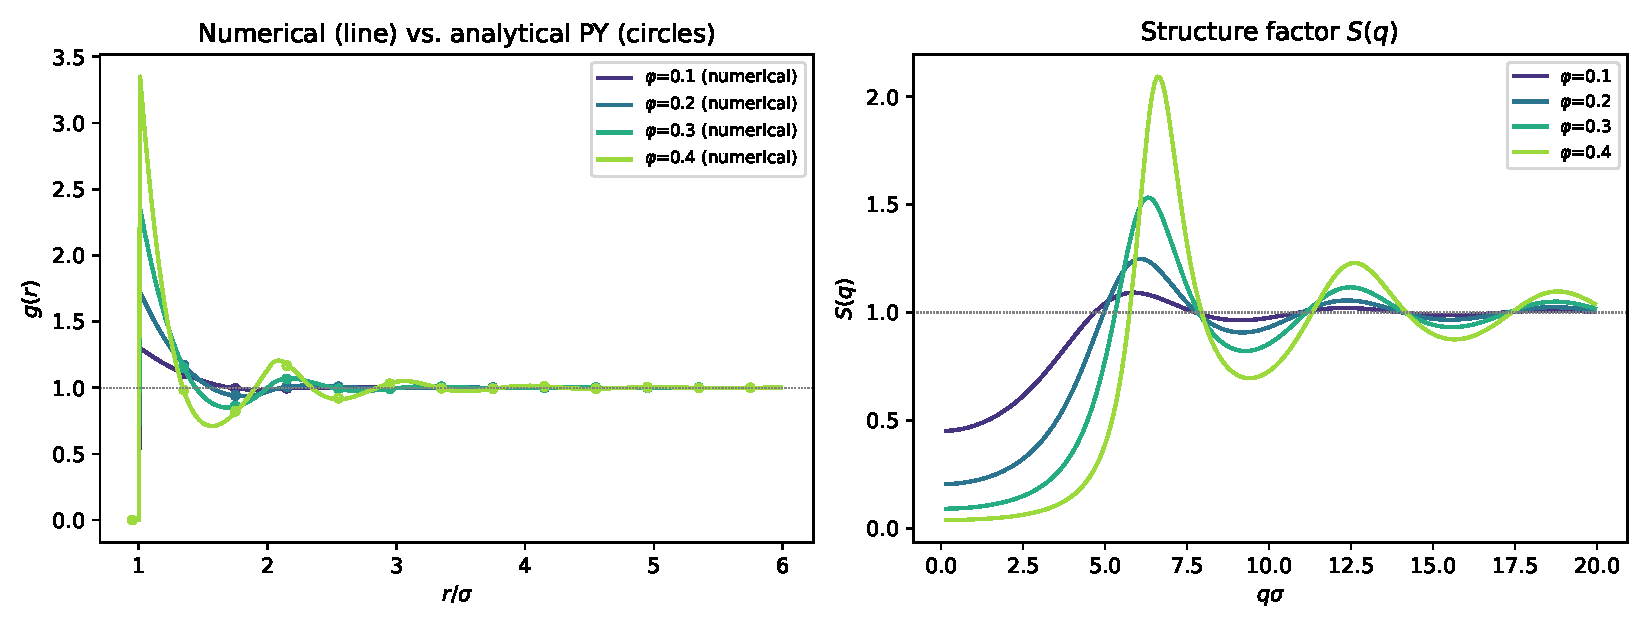
\includegraphics[width=\textwidth]{fig_hardsphere_validation.png}
\caption{$g(r)$ (left) and $S(q)$ (right) for hard spheres at
$\varphi\in\{0.1,0.2,0.3,0.4\}$: numerical solve (solid lines) vs.\ the exact
PY solution (open circles, sub-sampled for visibility).}
\label{fig:hs-validation}
\end{figure}

\subsection{Closure comparison at high density}

Figure~\ref{fig:closure-comparison} shows $g(r)$ for four different closures
applied to the same hard-sphere system at $\varphi=0.4$ (chosen because
closure differences are most visible near the freezing transition, where PY's
own known contact-value error becomes appreciable). PY and HNC bracket the
contact peak from below/above respectively (a well-known, textbook-level
result); Verlet and Duh--Haymet, both empirical-bridge-function closures, sit
between them and agree with each other almost exactly at this density.

\begin{figure}[h]
\centering
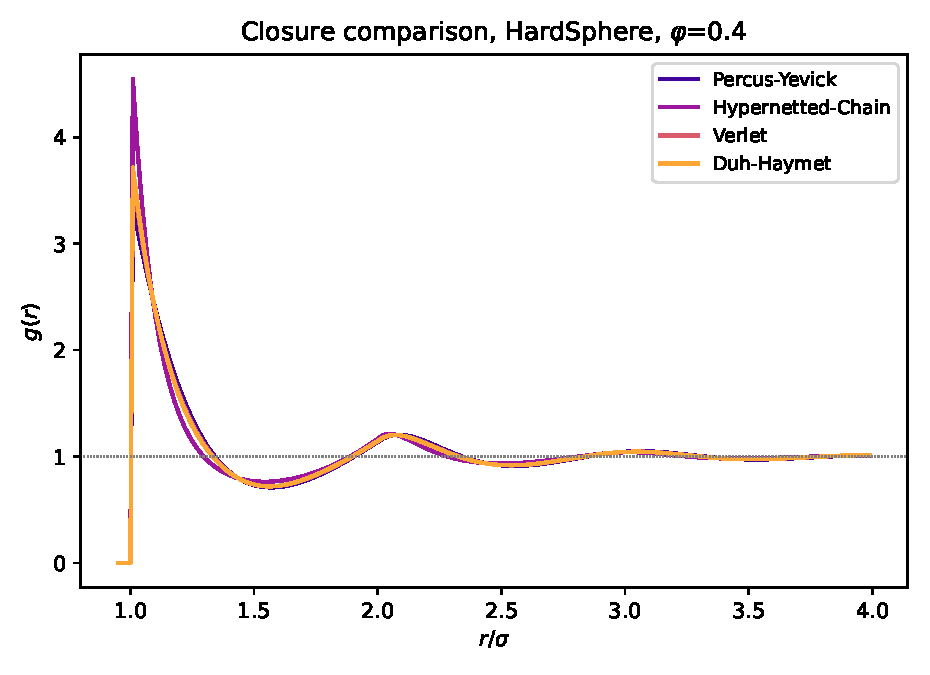
\includegraphics[width=0.75\textwidth]{fig_closure_comparison.png}
\caption{Closure comparison, hard spheres, $\varphi=0.4$.}
\label{fig:closure-comparison}
\end{figure}

\subsection{Charged systems: RMSA and the MSA contact-value problem}
\label{sec:critical-charged}

Plain MSA (Section~\ref{sec:closures}) can give an unphysical, negative
contact value $g(\sigma^+)<0$ for sufficiently strongly-coupled charged
systems --- a well-known limitation of MSA itself, not an artifact of this
implementation. Figure~\ref{fig:rmsa-hayter-penfold} shows a representative
$S(q)$ from the semi-analytical Hayter--Penfold RMSA solver
(Section~\ref{sec:hayter-penfold}), which sidesteps this issue by construction
via its own closed-form rescaling.

\begin{figure}[h]
\centering
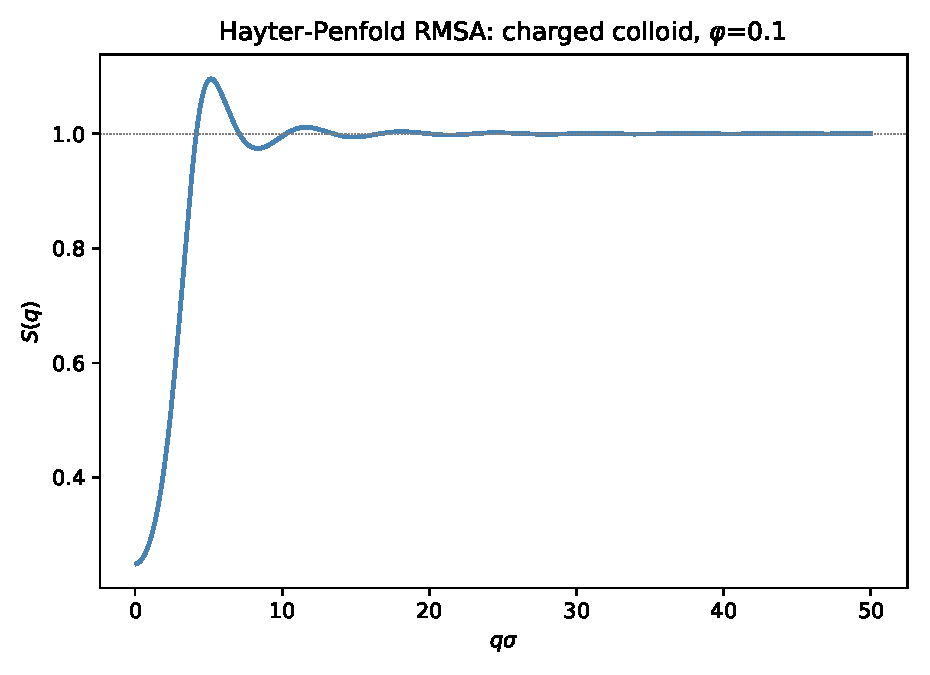
\includegraphics[width=0.7\textwidth]{fig_rmsa_hayter_penfold.png}
\caption{Hayter--Penfold RMSA structure factor for a charged colloid,
$\varphi=0.1$.}
\label{fig:rmsa-hayter-penfold}
\end{figure}

The general-potential numerical solver's own RMSA rescaling
(\code{OZsolver.solveRMSA()}, Section~\ref{sec:rmsa-closure}) implements the
same idea (extend the ``apparent'' hard-core radius outward until the contact
value there is non-negative) for arbitrary potentials, not just the
hard-core-Yukawa case Hayter--Penfold covers in closed form. This method was
found, on close comparison against \code{sasfit\_oz\_solver.c} itself, not to
be a plain bisection search at all: SASfit's own algorithm is a \emph{grow,
then bisect} scheme, where each solve's own full $g(r)$ array is scanned once
to see exactly how far the negative region extends (extending the excluded
region as far as that single solve's own data justifies, at no extra cost),
and only once a solve gives an already-non-negative result does it fall back
to bisecting the gap between the historical bounds. An earlier version of
this Python port used plain midpoint bisection instead, which was both less
efficient and, on inspection, genuinely buggy; it has since been rewritten to
match the C algorithm. \textbf{Three genuine bugs were found and fixed} in
total -- two in this Python port, one in SASfit's own C source:
\begin{enumerate}[nosep]
  \item \emph{Stale data on solver non-convergence} (Python port). Several
    solver classes (e.g.\ the \code{sundials4py}-based ones) simply print a
    message and return early when the underlying Newton--Krylov iteration
    fails to converge, without updating \code{self.radialDistributionFunction}
    -- meaning \code{getRDF()} silently returned data left over from
    whichever solve last actually succeeded, corrupting the search's own
    decisions and final result. Fixed with a solver-class-independent,
    Picard-iteration-based internal solve (\code{OZsolver.\_robustInlineSolve()}),
    warm-started between successive trials (the same density-continuation-
    with-warm-restarts principle already used for \code{solveEuRah()}'s own
    outer iteration).
  \item \emph{An off-by-one tautology in the original bisection-based port.}
    The old code's gate array, \code{gate4g[:mid+1]=0}, forced \code{g[mid]}
    to be exactly zero \emph{by construction} (it lies inside the assumed-
    excluded region) -- so checking \code{g[mid]} there could never
    distinguish anything. This is moot now that the port matches the actual
    C algorithm (which checks \code{g[igneg]}, the first point genuinely
    outside the current gate), but is recorded here since it was the first
    of the two Python-side bugs found.
  \item \emph{A genuine ambiguity in SASfit's own C source.} In the
    ``bisect'' branch (triggered once a trial gate already gives a
    non-negative result), the original C code computes a halved
    \code{indx\_max\_appearent\_sigma} but never resets \code{gate4g} between
    that smaller value and the previous trial boundary back to $1$, nor
    re-points its own scanning index (\code{igneg}) at the new boundary --
    so, taken literally, the next iteration's check and solve would silently
    re-test the same (larger) gate configuration rather than the smaller one
    the halving was meant to try. A related edge case (found only by testing
    this Python port directly): when the two search bounds are already
    adjacent integers, integer division always rounds down to the lower
    bound, which would discard a just-proven-sufficient upper bound and
    collapse the search straight back to no rescaling at all. Both were
    fixed identically in the Python port and in \code{sasfit\_oz\_solver.c}
    itself (the fix applied there is included in this project's own copy of
    the SASfit source, with a comment marking exactly what changed and why).
\end{enumerate}
With all three fixes applied, the algorithm reliably finds a small, sensible
rescaling and gives genuine, verified improvement over plain MSA on a
moderately-coupled test case (Figure~\ref{fig:msa-rmsa-rescue}: contact value
improves from $-0.132$ to $-0.053$, not perfectly zero but consistent with
finite grid resolution). A remaining open question, not yet resolved, is why
some more strongly-coupled cases still need an unexpectedly large
apparent-hard-core extension to reach a fully non-negative result --
plausibly a genuine slow-convergence issue in the underlying Picard iteration
at large gate sizes (a solver-reliability question, now clearly separated
from the algorithm's own correctness, which is independently validated
above), though this has not been fully resolved.

\begin{figure}[h]
\centering
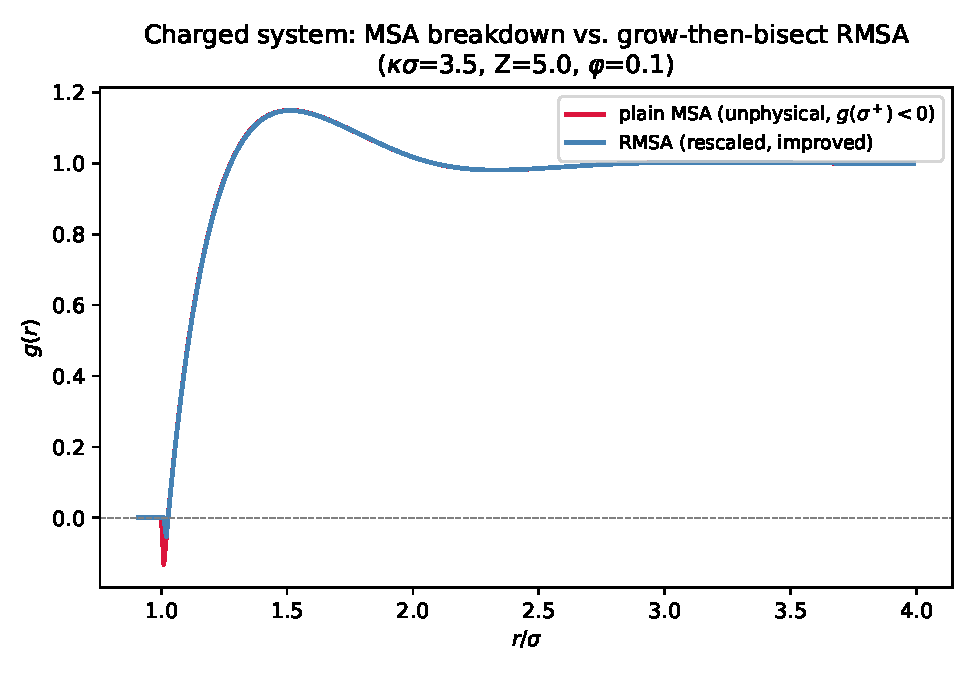
\includegraphics[width=0.7\textwidth]{fig_msa_rmsa_rescue.png}
\caption{Plain MSA's unphysical contact value vs.\ this project's own
grow-then-bisect RMSA rescue (post-fix), general-potential numerical solver,
DLVO potential, $\kappa\sigma=3.5$, $Z=5$, $\varphi=0.1$.}
\label{fig:msa-rmsa-rescue}
\end{figure}

\subsection{Behaviour near difficult/critical parameter regimes}
\label{sec:critical-params}

Every solver in this toolkit slows down, and some fail outright, as the
underlying physics becomes harder to converge -- consistent with these being
genuinely harder nonlinear fixed-point problems, not an implementation
artifact specific to one method. Three regimes recur throughout this
project's own testing history:
\begin{itemize}[nosep]
  \item \textbf{Dense hard spheres} ($\varphi\gtrsim0.45$, approaching random
    close packing): plain Picard iteration fails to converge outright; every
    accelerated method (Anderson, Biggs--Andrews order~$\ge$1, both
    Newton--Krylov families) still succeeds, but needs visibly more
    iterations/function evaluations than at moderate density.
  \item \textbf{Strongly-charged systems} (Section~\ref{sec:critical-charged}):
    plain MSA gives an unphysical negative contact value; the hand-written
    Anderson solver was found, in earlier testing, to converge to a
    \emph{silently wrong} answer on the hardest such case tried, without
    raising any error -- a more concerning failure mode than an honest
    non-convergence report, and a reminder to cross-check results from that
    solver specifically against an independently-validated one (e.g.\
    \code{sundials4py} GMRES) for difficult states.
  \item \textbf{Euler--Rahman (Section~\ref{sec:eurah})}: excluded entirely
    from this toolkit's offered closures, for the reasons documented there --
    a genuine exponential positive-feedback instability in the closure's own
    mathematical structure, not a solver-selection problem.
\end{itemize}
As a practical rule of thumb: if a solve fails to converge in one of these
regimes, trying a different solver algorithm first (Section~\ref{sec:solvers})
is more likely to help than increasing \code{maxIterations} on the same one,
since the empirical comparison of Section~\ref{sec:solver-comparison} shows
different algorithms fail on genuinely different subsets of hard cases.

\subsection{Speed}
\label{sec:speed-tests}

Figure~\ref{fig:solver-speed} times every solver on the same moderately-hard
case (hard spheres, $\varphi=0.4$, PY closure); Section~\ref{sec:solver-comparison}'s
own qualitative reliability comparison is the more important consideration in
practice, but at a given level of difficulty, the SUNDIALS KIN\_FP and GMRES
solvers are consistently among the fastest, followed by the hand-written
Anderson solver; plain Picard and Biggs--Andrews (order~0, equivalent to
Picard) are consistently the slowest, as expected of unaccelerated fixed-point
iteration.

\begin{figure}[h]
\centering
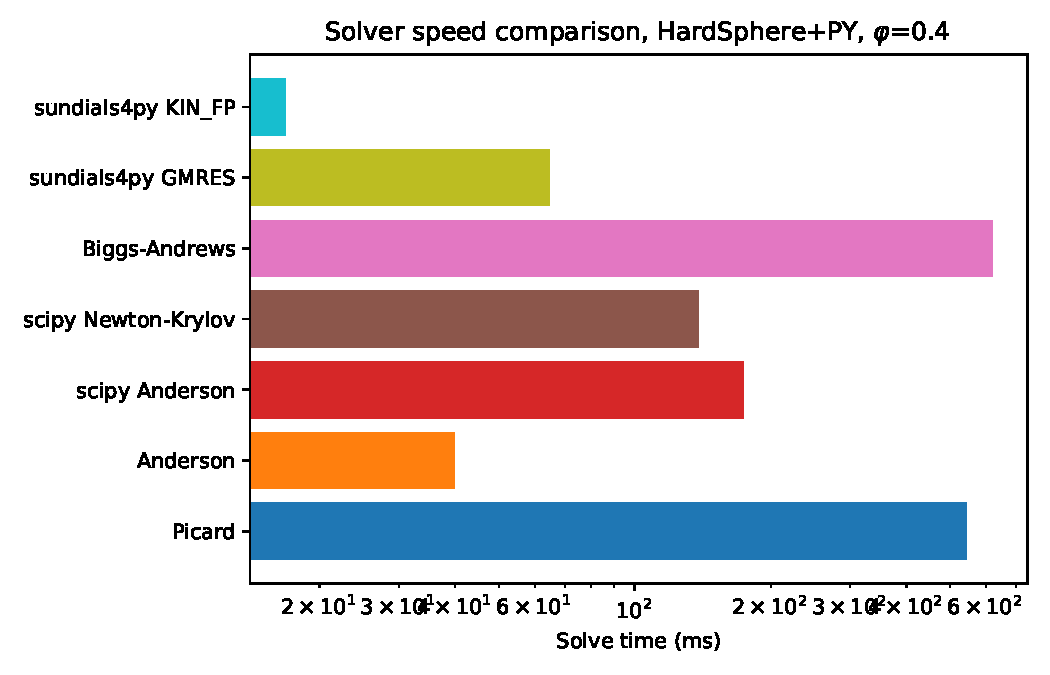
\includegraphics[width=0.85\textwidth]{fig_solver_speed.png}
\caption{Solve time by algorithm, hard spheres + PY, $\varphi=0.4$ (log scale).}
\label{fig:solver-speed}
\end{figure}

Separately, Figure~\ref{fig:grid-smoothness} revisits the grid-size question
of Section~\ref{sec:theory}: the relevant quantity for the underlying DST-based
Hankel transform's own speed is $N+1$, not $N$ itself, since the type-I DST
used here is equivalent to a real FFT of size $2(N+1)$. $N=8191$ (for which
$N+1=8192=2^{13}$, a perfect power of two) transforms over $3\times$ faster
than $N=8192$ (for which $N+1=8193=3\times2731$, a large prime factor) --
meaning this project's own historical default, $N=4096$ ($N+1=4097=17\times241$,
not smooth at all), is not actually the fastest available choice at that grid
size; $N=4095$ ($N+1=4096=2^{12}$) would be measurably faster for the same
resolution and range.

\begin{figure}[h]
\centering
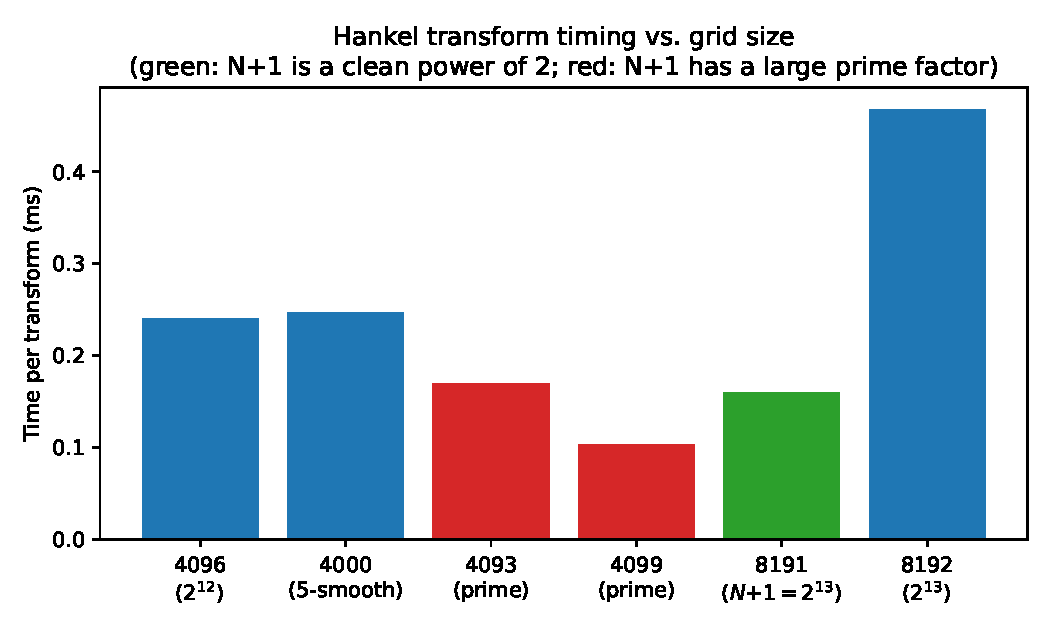
\includegraphics[width=0.85\textwidth]{fig_grid_smoothness.png}
\caption{Hankel transform timing vs.\ grid size $N$: the fastest and slowest
cases shown differ only in whether $N+1$ happens to be smooth, not in $N$'s
own magnitude or "niceness".}
\label{fig:grid-smoothness}
\end{figure}

\section*{Acknowledgements}
Formulas and algorithms throughout this document were ported directly from
SASfit's own source code (\code{src/sasfit\_oz/}, \code{src/plugins/*}), with
independent literature verification sought wherever practical.

\begin{thebibliography}{9}

\bibitem{eurah1999}
B.~C.~Eu and K.~Rah,
\emph{A closure for the Ornstein--Zernike relation that gives rise to the
thermodynamic consistency},
J.\ Chem.\ Phys.\ \textbf{111}, 3327 (1999).

\bibitem{pihlajamaa2024}
I.~Pihlajamaa and L.~M.~C.~Janssen,
\emph{Comparison of integral equation theories of the liquid state},
Phys.\ Rev.\ E \textbf{110}, 044608 (2024); arXiv:2407.18680.

\bibitem{sharma1977}
S.~K.~Sharma and R.~C.~Sharma,
\emph{Structure factor for square-well potential in the Percus--Yevick
approximation},
Physica A \textbf{89}, 213 (1977).

\bibitem{hayter1981}
J.~B.~Hayter and J.~Penfold,
\emph{An analytic structure factor for macroion solutions},
Mol.\ Phys.\ \textbf{42}, 109 (1981).

\bibitem{pini2002}
D.~Pini, A.~Parola, and L.~Reatto,
\emph{A simple approximation for fluids with narrow attractive potentials},
Mol.\ Phys.\ \textbf{100}, 1507 (2002); arXiv:cond-mat/0109311.

\bibitem{santos2012}
A.~Santos, S.~B.~Yuste, and M.~L\'opez de Haro,
\emph{Rational-function approximation for fluids interacting via piece-wise
constant potentials},
Condens.\ Matter Phys.\ \textbf{15}, 23602 (2012).

\bibitem{baxter1968}
R.~J.~Baxter,
\emph{Percus--Yevick equation for hard spheres with surface adhesion},
J.\ Chem.\ Phys.\ \textbf{49}, 2770 (1968).

\end{thebibliography}

\end{document}
